\section{Hvordan det er at være med i Coding Pirates}
\begin{frame}
\frametitle{Hvad laver vi? (i GameDev)}
    \newcommand{\nodenames}{
        Engine, Logik, Assets, Design, Historiefortælling, Samarbejde
    }
    \begin{center}
    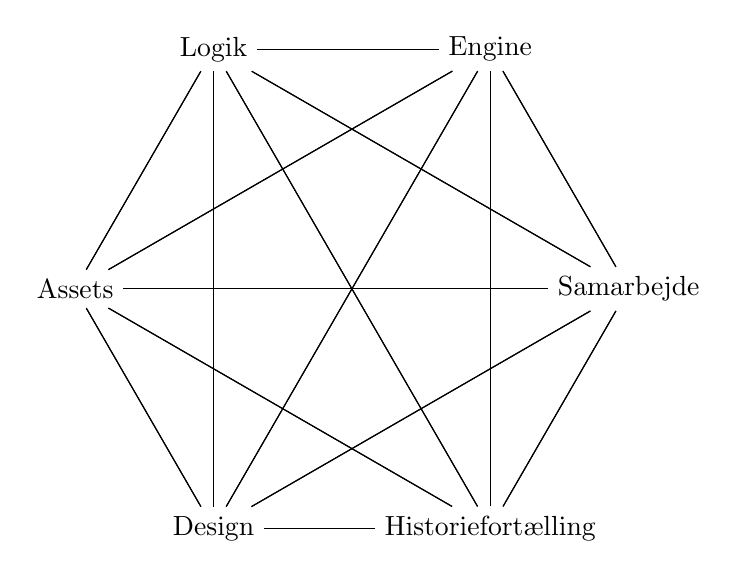
\begin{tikzpicture}
        % Draw boxes (Vertices/Nodes)
        \foreach [count=\i] \x in \nodenames{
            \node (\x) at(\i*60:10em) {\x};
        }
        % Draw box connects (Edges) 
        \foreach \x in \nodenames{
            \foreach \y in \nodenames{
                \ifx\x\y
                    % Don't create loop on every node 
                \else
                    \draw (\x) -> (\y);
                \fi
            }
        }
    \end{tikzpicture}
    \end{center}
\end{frame}

\begin{frame}
\frametitle{Hvordan kan man være med?}
    \begin{tikzpicture}
        Lad x være dig!
        \graph[branch down=5em]{
            A[at={(0,0)}, as={RigtigAlder(x) = $x>=12$år OG $x<= 17$år}];
            B[at={(0,1)}, as={InteresseretIComputerSpil(x)}];
            C[at={(0,2)}, as={FriOnsdagAften(x)}];
            D[at={(0,3)}, as={ErNysgerrigPåSoftware(x)}];
            E[at={(0,4)}, as={KanTilmeldeDig(x) = Har500kr(x) OG KanFindeCodingPirates.dk(x)}];
            F[at={(0,9)},as={VilNogetAndet(x)}];

            {A,B,C,D,E} -> F;
        };
    \end{tikzpicture}
\end{frame}

\begin{frame}
\frametitle{Demo og hvordan en game engine ser ud!}
Et produkt fra gamedevafdelingen, som man kan finde på steam!
\begin{figure}
    \href{https://store.steampowered.com/app/1589450/Frogiee/}{\includegraphics[width=\textwidth, keepaspectratio]{/home/madshebsgaard/Projects/CodingPiratesOutReach/assets/pictures/Frogiee_1920x1080.jpg}}
    \caption{Platformerspillet Frogiee af Peter Kragh og Thomas Lauridsen (2021)\cite{Pirates_frogiee}}
    \label{fig:frogiee_screenshot}
\end{figure}
\end{frame}
